\documentclass[c,8pt,xcolor...,x11names]{beamer}
\usepackage{icclslides}
\usepackage[latin1]{inputenc}
\usepackage[british]{babel}
\usepackage{amssymb}
\usepackage{latexsym}
\usepackage{rotate}
\usepackage{tikz}
\usepackage{verbatim}
\usepackage{colortbl}
\usepackage{booktabs}
\usepackage{ulem}
% \usepackage{arydshln}
%\usepackage{pdfpages}hord
\usepackage{graphicx} 
\usepackage{tikzsymbols}
\usepackage{tikz}
\usepackage{subcaption}
\usepackage[export]{adjustbox}
\usepackage{pdfpages}
\usetikzlibrary{positioning}

\tikzstyle{ele} = [circle, text centered, minimum width=1em, minimum height=3ex]

%% Uncomment to activate navigation symbols in the lower right of the pages:
\setbeamertemplate{navigation symbols}{}
%\setbeamercovered{transparent}

\renewcommand{\Myauthor}{Martin R\"obke}
\renewcommand{\Mytitle}{Visualizing Dynamic Programming \newline
	On Tree Decompositions}
\usepackage{showexpl} 

\lstloadlanguages{[LaTeX]Tex} 
\lstset{% 
     basicstyle=\ttfamily\small, 
     commentstyle=\itshape\ttfamily\small, 
     showspaces=false, 
     showstringspaces=false, 
     breaklines=true, 
     breakautoindent=true, 
     captionpos=t 
} 

\begin{document} 
\begin{frame}
\customtitle
\begin{list2}
\item {\sc What} is this about?
\item {\sc Who} benefits from visualization?
\end{list2}
\end{frame}

%%%%%%%%%%%%%%%%%
 \section{About me} % taken from Marek Seliger, Matthias Gerdts


 \begin{frame}
  \frametitle{About me}
	
 {\color{blue}Martin R\"obke}
 \medskip

\begin{minipage}{0.6\textwidth}
    \begin{itemize}
    % \item[$\bullet$] born in Dresden
    \item[$\bullet$] studying Bachelor CS
    \begin{itemize} \smallskip
    \item[$\bullet$] started studying physics at the TU Dresden
    \item[$\bullet$] did like logic and visualization more, so switched the faculty ~ {\color{orange}\Winkey}
	\end{itemize}
    \end{itemize}
\end{minipage}\hfill
\begin{minipage}{0.35\textwidth}
	\begin{figure}[H]
			
\includegraphics[height=0.33\textheight]{images/Martincrop.jpg}
	\end{figure}
\end{minipage} 
\medskip
 {\color{blue}How did I get to work with my supervisor Johannes Fichte?}
\begin{center}
	\quad 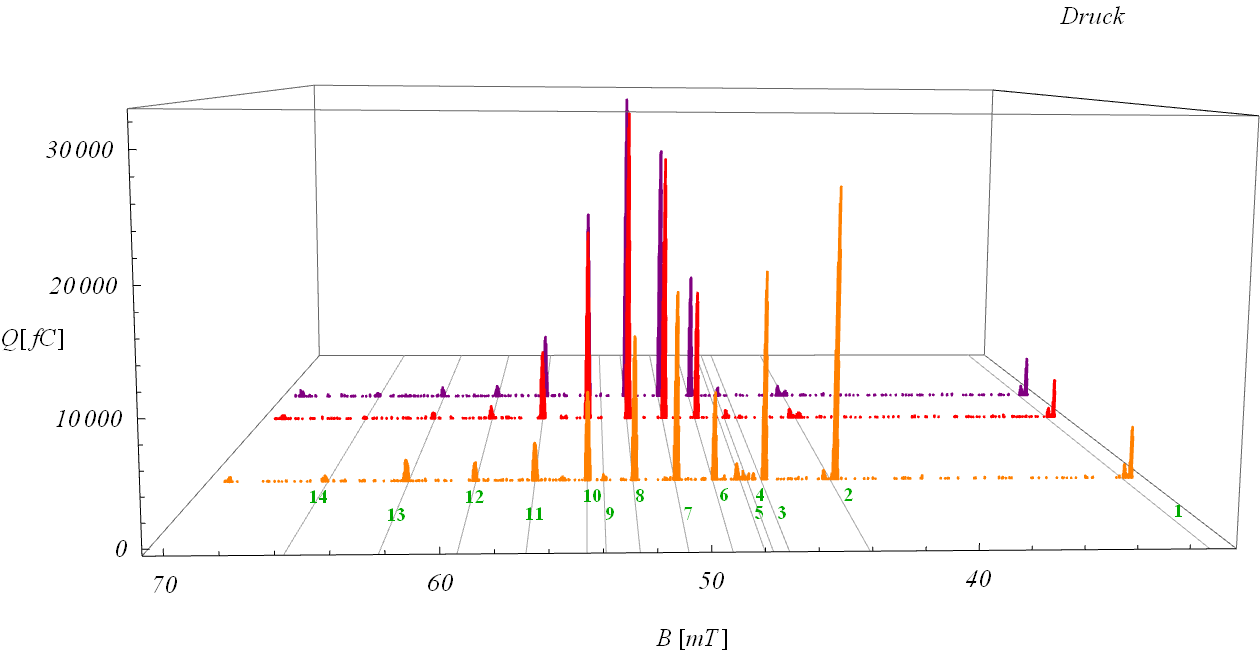
\includegraphics[width=.3\linewidth]{images/3DLabelsgrossGrun.png}\qquad 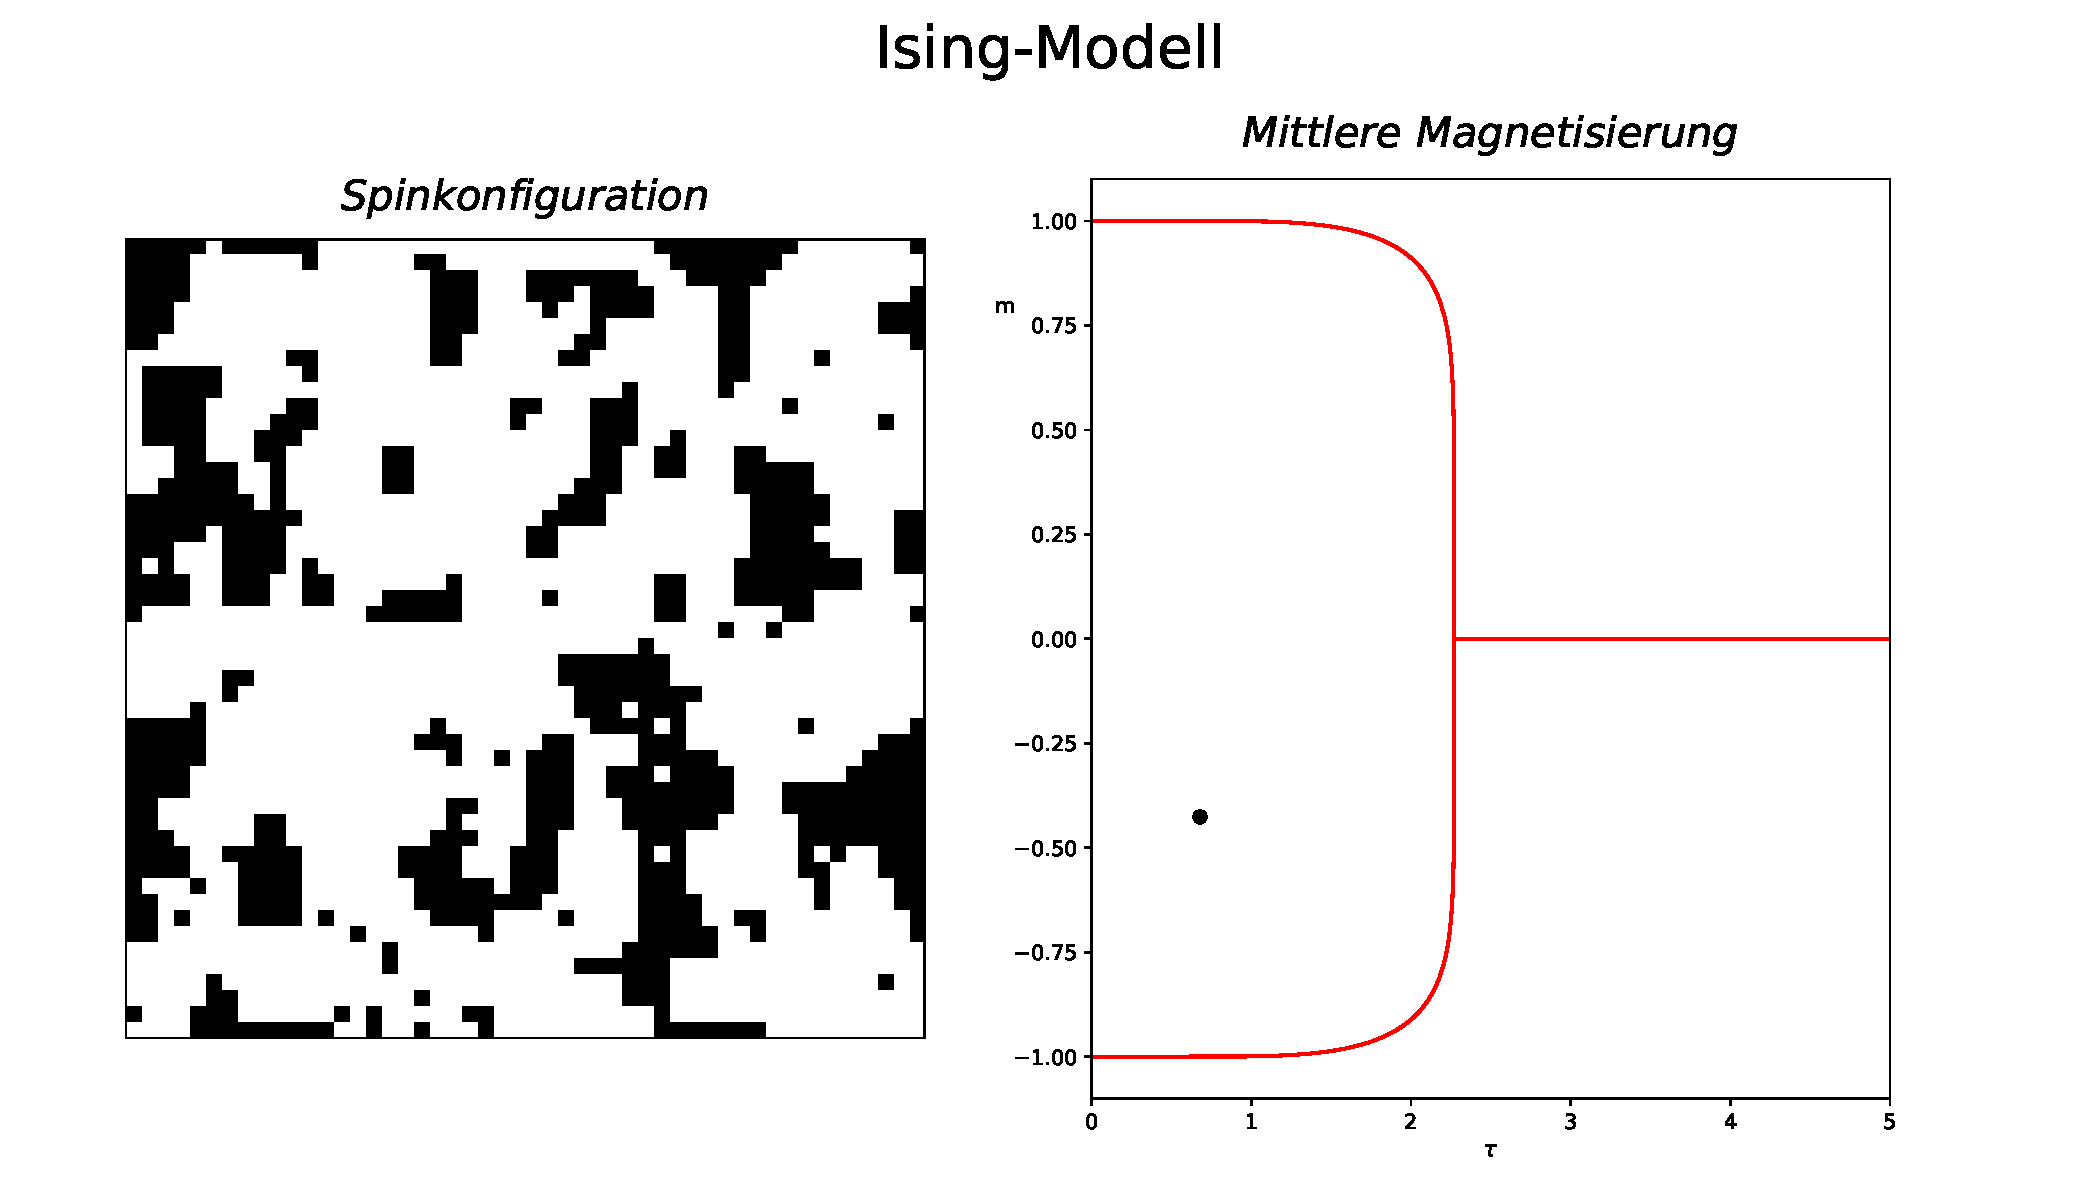
\includegraphics[width=.3\linewidth]{images/IsingModell.pdf}
\end{center}
\end{frame}

%%%%%%%%%%%%%%%%%%%%%%
\section{Motivation}

\begin{frame}
	\frametitle{Motivation}
	\begin{minipage}{0.7\textwidth}% \textbf{\color{blue}Previous work:} 
	\medskip
	\begin{itemize}
		%Chapter 1IntroductionModeling and solving real-world problems are two cornerstones ofArtificial Intelligence(AI).  In  particular,  the  sub-area  ofAutomated  Reasoningtackles  these  challenges  bydeveloping modeling languages to encode real-world problems as well as algorithms tosolve them.  Here we focus on approaches that are mainly based on mathematical logicthat have already proven successful on a wide range of real-world applications such asplanning, verification, and robotics (see e.g., [50]). 
		%http://www.cs.toronto.edu/~horst/cogrobo/papers/phdthesis-horst.pdf
		\item SAT-Problem is NP-complete \quad \#SAT is \#P-complete

		\begin{itemize}
				\item Problem with huge instances
		\end{itemize}

		%Using customized algorithms and datastructures and highly parallel hardware
		\item Customized algorithms, data-structures, hardware
	\end{itemize}

	\medskip

	\textbf{\color{blue}Why visualization?}\medskip
	\begin{center}
		{\color{blue}$\rightarrow$ trace and document the customization}
	\end{center}
	
	\textbf{\color{blue}Outlook:} \medskip
	\begin{itemize}
		\item Improve and streamline the visualization process % API, diff. programs etc. 
		\item Implement debug-output in existing solvers
		%Enable
		\item Even more dynamic possibilities 
	\end{itemize}
	\end{minipage}\hfill
	\begin{minipage}{0.28\textwidth}
		\begin{figure}[H]
			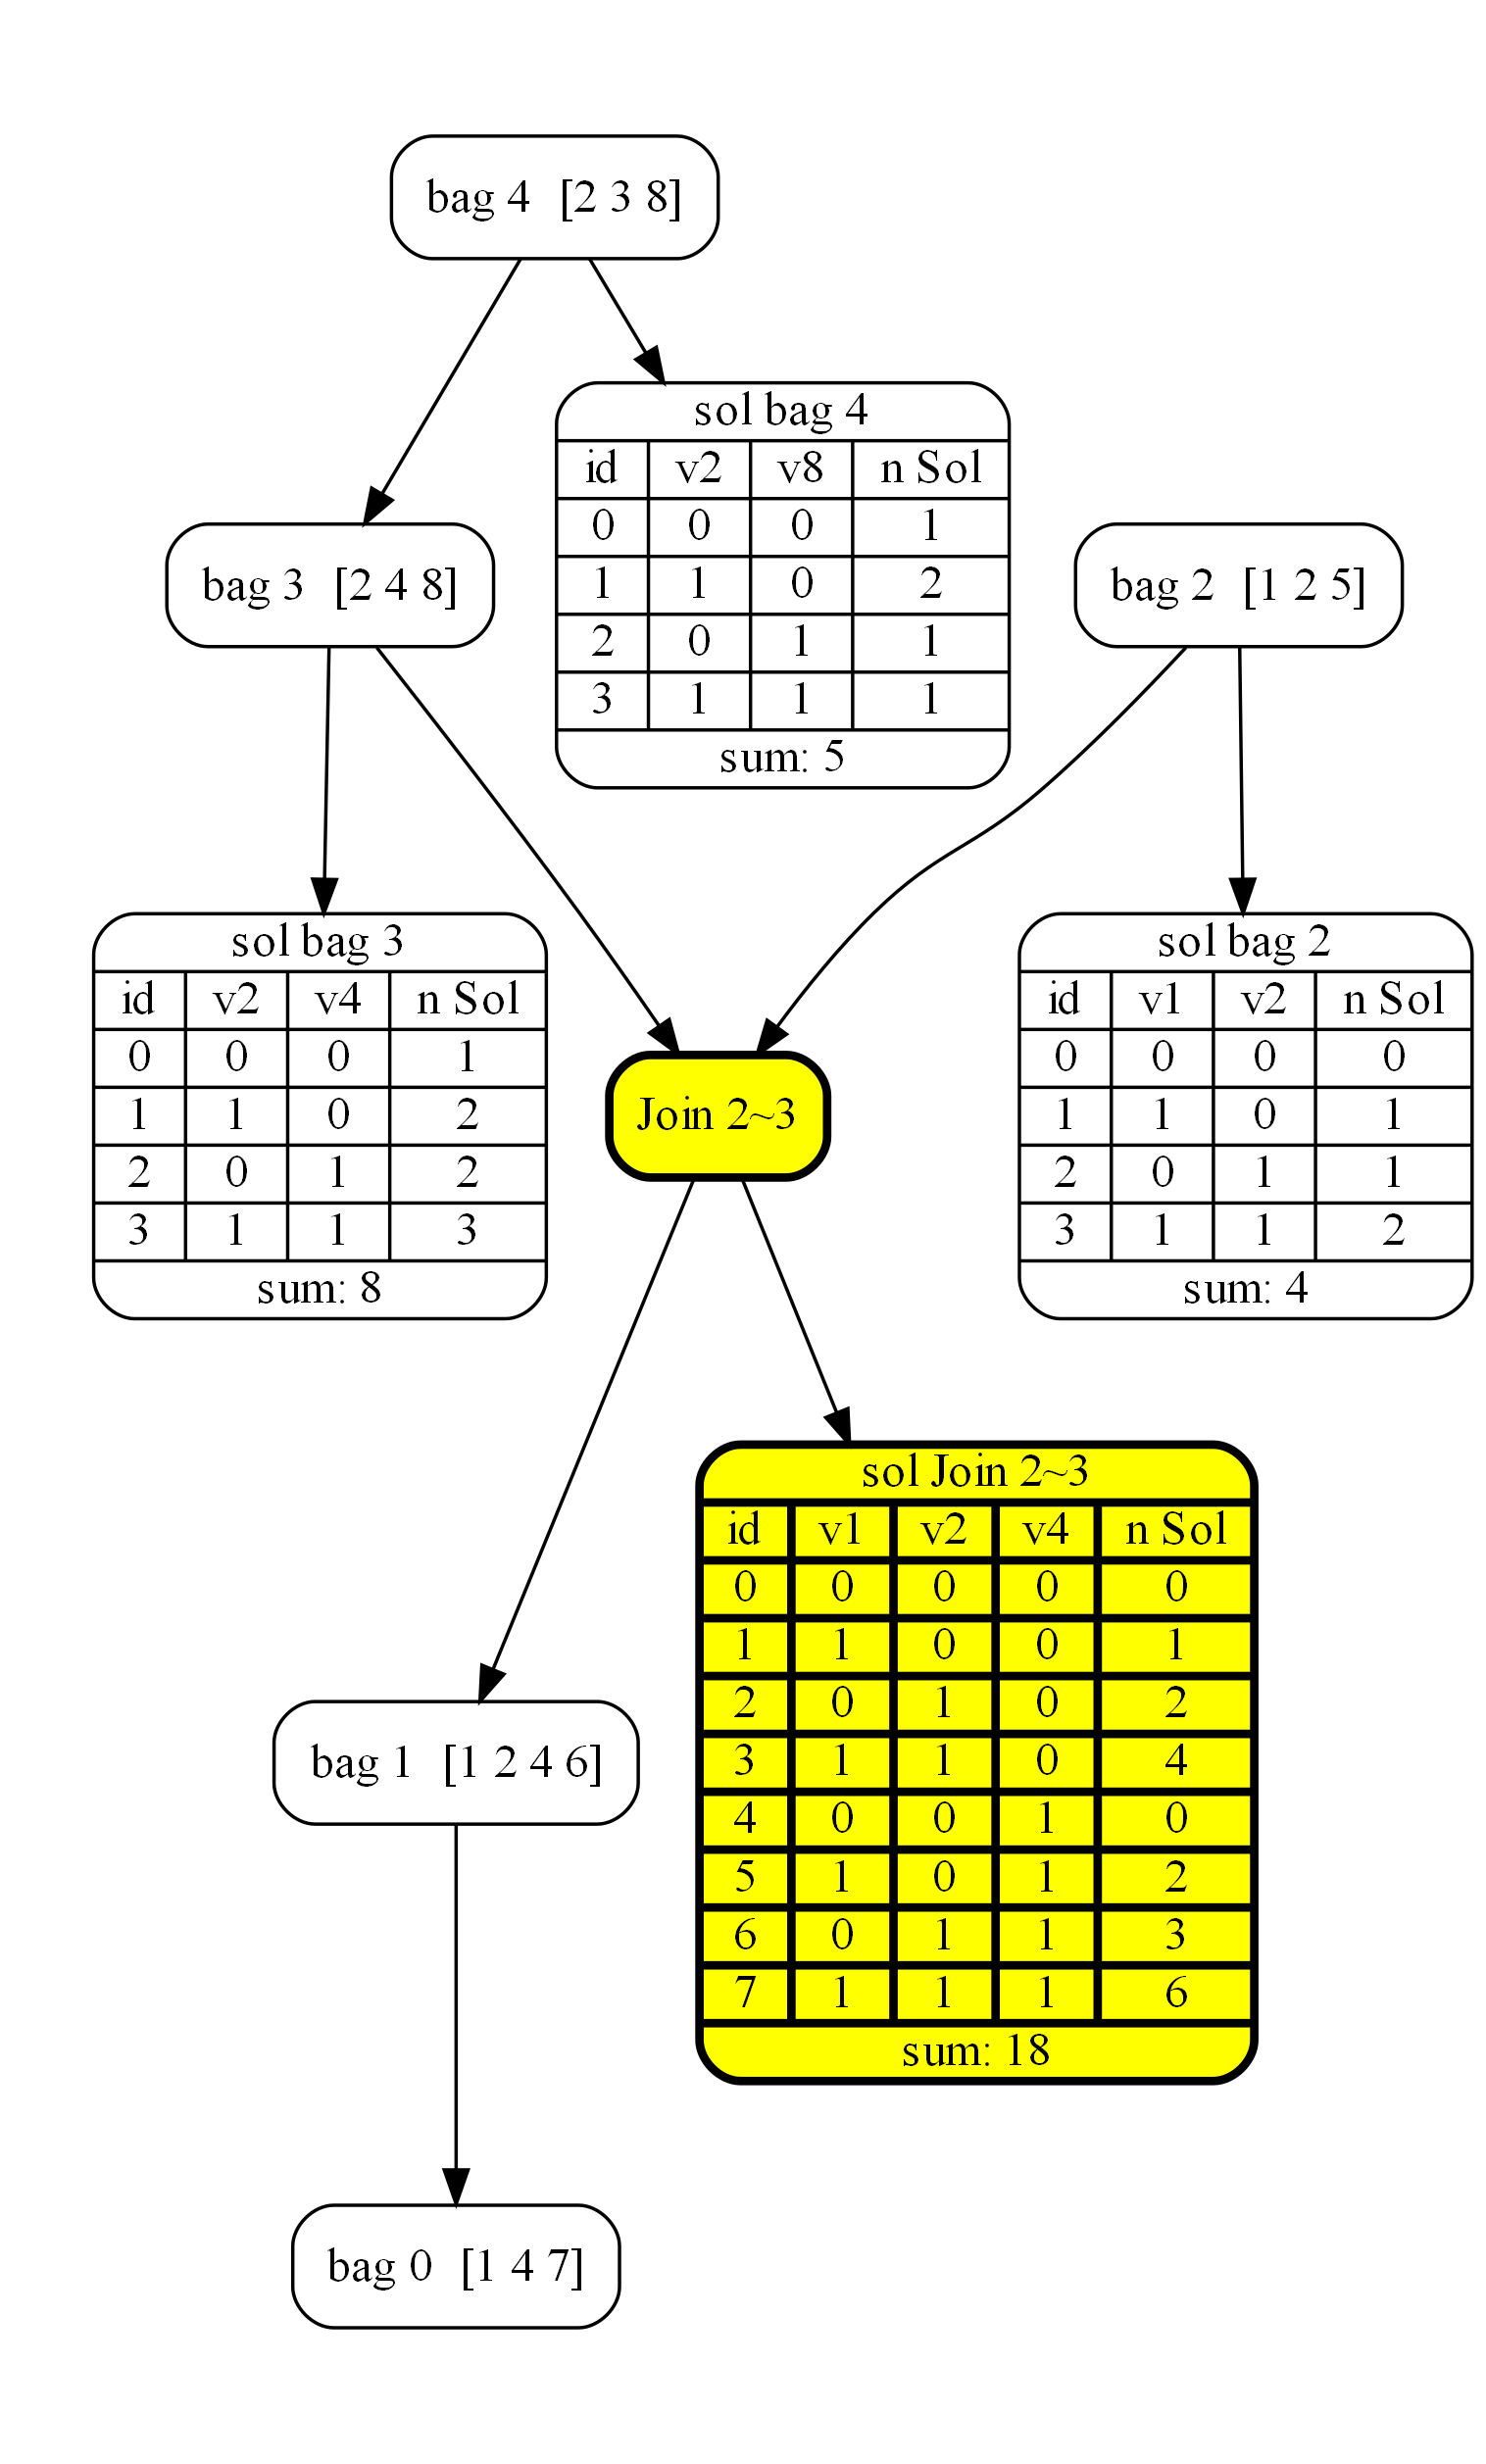
\includegraphics[width=\linewidth]{images/g41DigraphProgress6.png}
			\caption{\label{fig:g416} Example of a \#SAT run with DP}
		\end{figure}
	\end{minipage} 

\end{frame}

%%%%%%%%%%%%%%%%%%%%%
\section{Background}
\subsection{Different extensions of logic}
\begin{frame}
	\frametitle{Background}
	\begin{figure}
		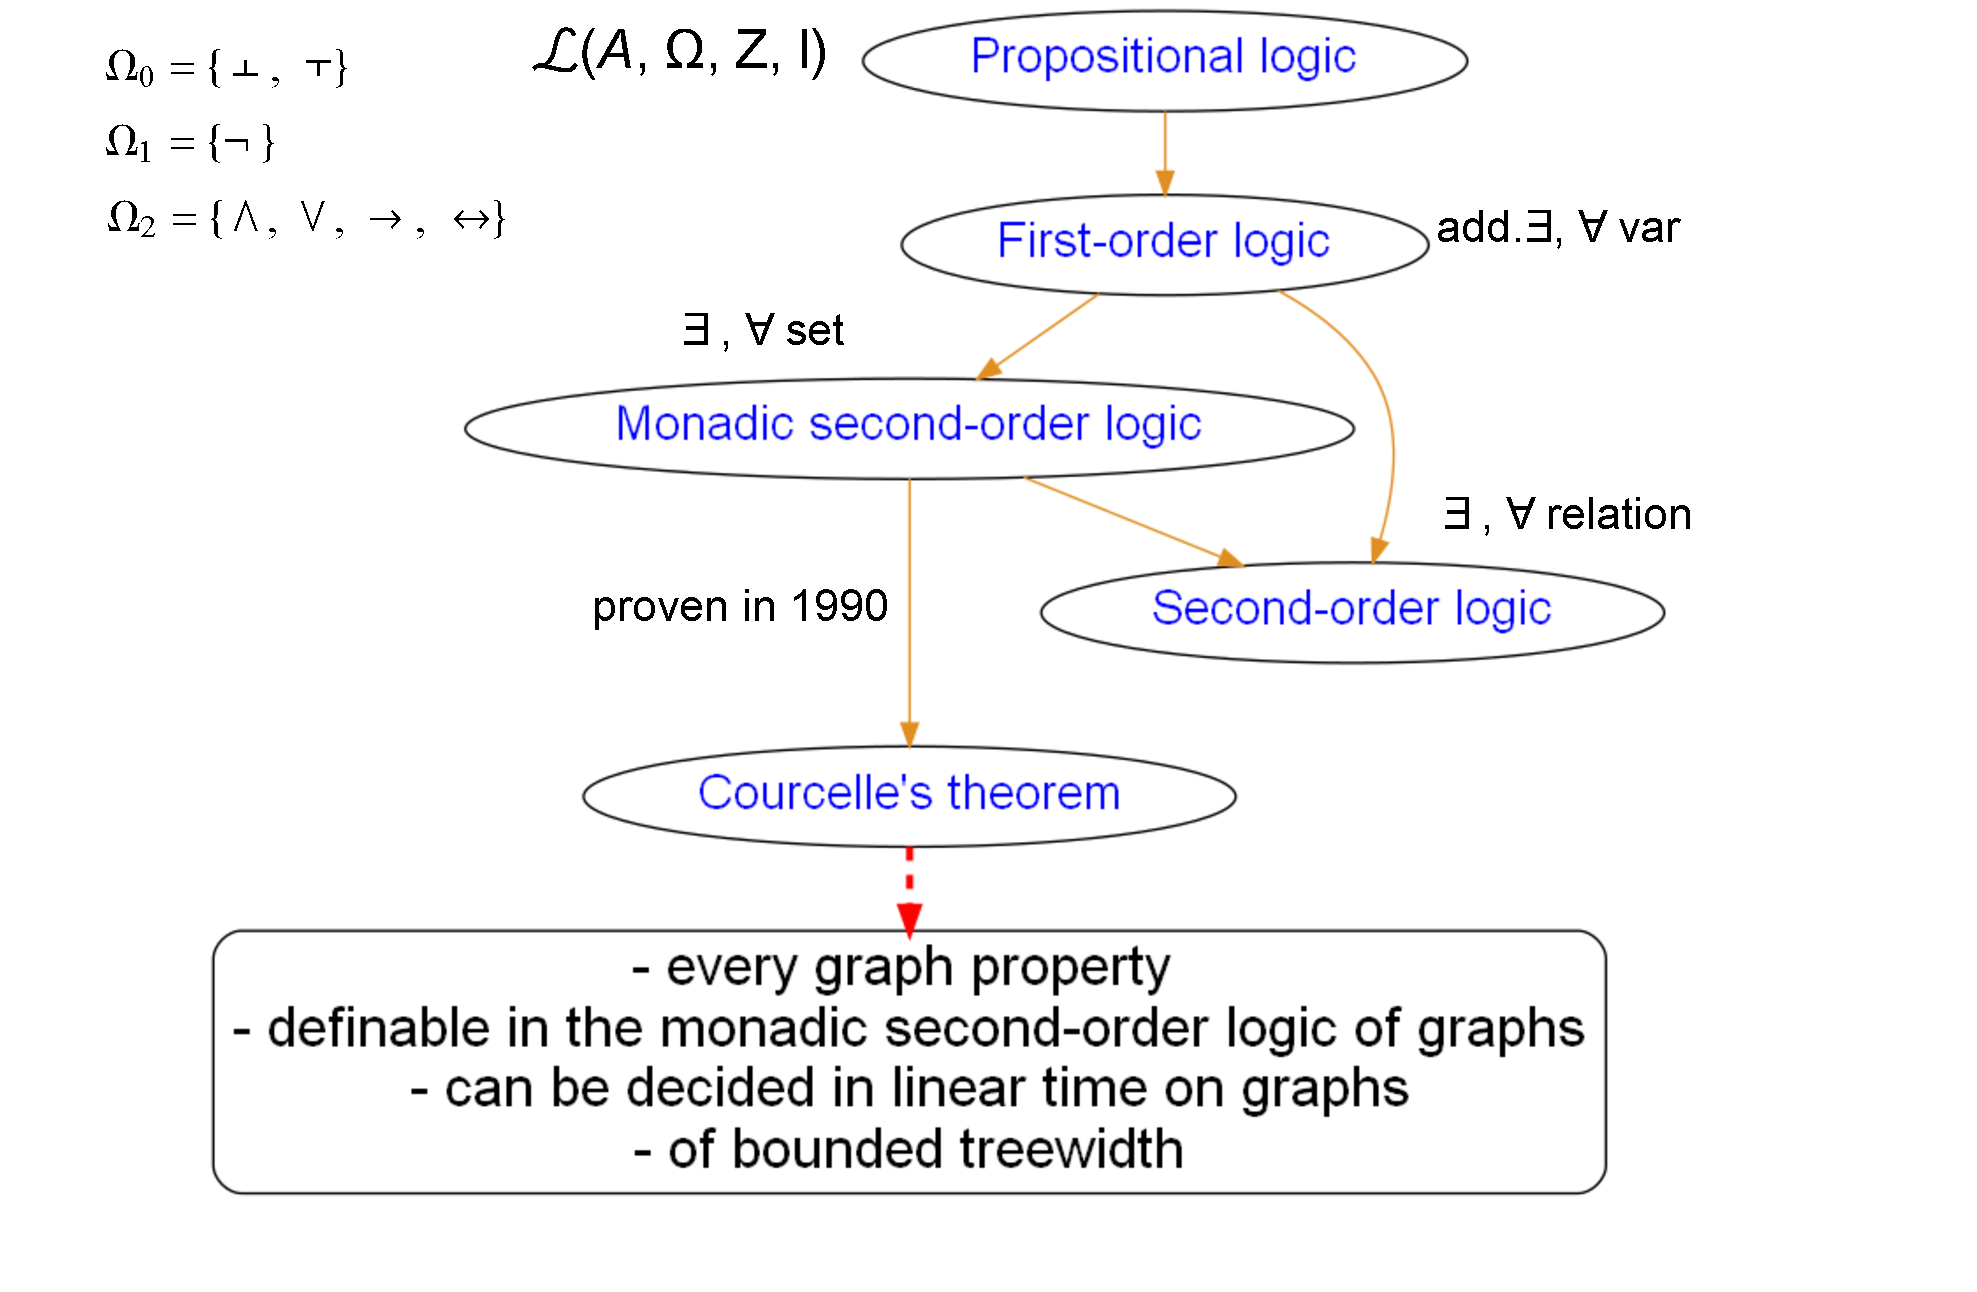
\includegraphics[height=0.9\textheight]{images/DifferentLogicgraph3.pdf}
	\end{figure}
\end{frame}
%%
\subsection{Example Vertex cover}
\begin{frame}
\frametitle[Vertex Cover]{Example: Vertex-Cover problem}

%We take an undirected graph 
%\begin{center}
%	We take an undirected graph	\textbf{G} = (\textbf{V}, \textbf{E})
%\end{center}
%where \textbf{V} is the set of nodes and \textbf{E} the set of edges, each between two elements of \textbf{V}. 
For the graph \textbf{G~=~(V,~E)} we want to compute a set C $\subseteq V(G)$ such that \emph{from every edge} $\{u, v\}$ there is \emph{at least one} of $u$ or $v$ in C. \smallskip 

\begin{figure}
	\centering
	\begin{minipage}{0.45\textwidth}
		\centering
		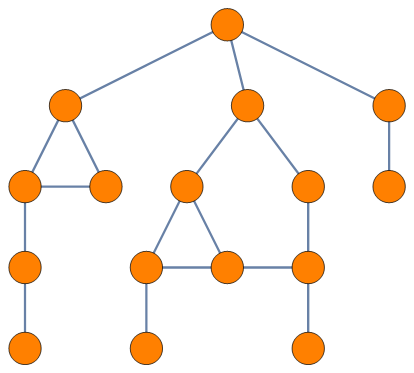
\includegraphics[width=0.6\textwidth]{"images/threeGraph1.png"}
		\caption{Example undirected graph \textbf{G}} 
	\end{minipage}
	\begin{minipage}{0.45\textwidth}
		\centering
		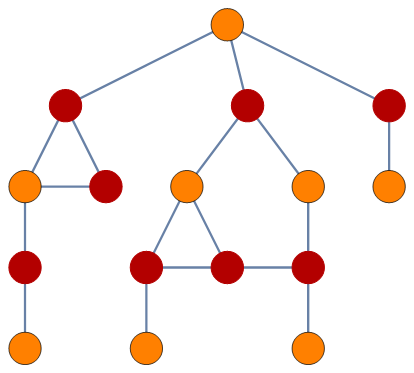
\includegraphics[width=0.6\textwidth]{images/threeGraphOptimal.png} 
		\caption{Minimal VC of \textbf{G}} 
	\end{minipage}
\end{figure}

%The size of the vertex cover is the number of vertices in it.
\hspace*{0.1\textwidth}
\begin{minipage}{0.8\textwidth}
	\begin{center}
		$\exists S: ~\forall \{u,v\} \in E: (u\in S \vee  v\in S)$
	\end{center} \medskip
	{\color{blue}for a given $k {\small \in} \mathbb{N}$: \\Deciding whether the graph has a vertex cover of size k is NP-complete.
	%{\color{blue}Finding the \emph{smallest} of these sets is the optimization version % (how large is the smallest set?) 
	%	of a NP-complete decision problem. %(is there a vertex cover of size \textit{k}).
	}

\end{minipage}
\end{frame}
%%
\subsection[Courcelle]{Courcelle's theorem}
\begin{frame}
	\frametitle{Courcelle's theorem}
	
	\begin{quotation}
		Every graph property definable in monadic second-order logic (MSO) is decidable in linear time on graphs of bounded treewidth. \\
		\hfill {\small Courcelle, Bruno (1990)}\footnote{Courcelle, Bruno "The monadic second-order logic of graphs. I. Recognizable sets of finite graphs",\\ Information and Computation, 85 (1990) no. 1: 12-75}
	\end{quotation}

	\medskip 
	For all $k \in \mathbb{N}$ and MSO-sentences F is the decision problem for a given graph G, whether $G \models F$ is true, in time $2^{p(tw(G))} \cdot |G|$ with a polynom p decidable.
	\medskip 
	\begin{itemize}
		
		\item \emph{drawback:} still expensive ($2^{p(tw G)}$, $2^{2^{(\#Q)}}$, large constants) \smallskip 
		\item usage:
		
\end{itemize}
\begin{figure}
	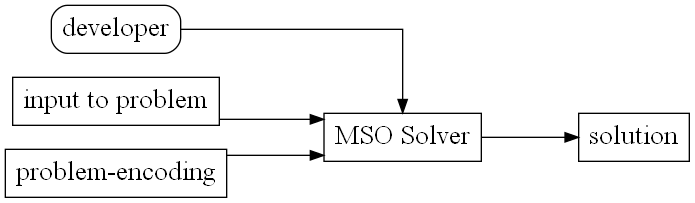
\includegraphics[height=0.2\textheight]{images/UsageCourcelle.gv.png}
	\caption{Implementation of the theorem}
\end{figure}
\end{frame}
%%
\subsection{\#SAT and WMC}
\begin{frame}
	\frametitle{(Weighted) Model-Counting}
	\begin{minipage}{0.75\textwidth}
% https://en.wikipedia.org/wiki/Sharp-SAT#Intractable_special_cases
	\vspace{.2\textheight}
	{\color{blue} The \#SAT Problem} \\
	Input: boolean formula \textbf{F} \\
	Output: the number of satisfying assignments for \textbf{F}
	
	\bigskip
	{\color{blue} The Weighted Model Counting Problem}
	\begin{itemize}
		%\item $w(lit=\top ) \in [0,1], \quad w(lit=\perp) = 1-w(lit=\top)$
		\item $w(lit) \in [0,1], \quad w(� lit) = 1-w(lit)$
		\item $w(assignment) = \prod_{lit} w(lit)$
		\item $WMC(formula) = \sum_{\small satisfying~~ assignments} w(assignment)$
	\end{itemize}
	\end{minipage}\hfill
	{\raisebox{-0.7\height}{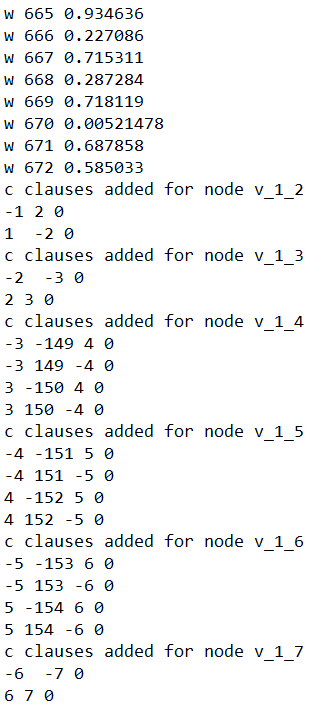
\includegraphics[width=0.23\textwidth]{images/ExampleCNFw.png}}}
\end{frame}
\begin{frame}
	\frametitle{Example for WMC}
	\smallskip
	\begin{itemize}
		\item {\color{blue} Example set of CNF-clauses:}\smallskip\\
		{\tiny $\{\text{c1}=\{\text{v1},\text{v3},\neg \text{v4}\},\text{c2}=\{\neg \text{v1},\text{v6}\},\text{c3}=\{\neg \text{v2},\neg \text{v3},\neg \text{v4}\},\text{c4}=\{\neg \text{v2},\text{v6}\},\text{c5}=\{\neg \text{v3},\neg \text{v4}\},\text{c6}=\{\neg \text{v3},\text{v5}\},\text{c7}=\{\neg \text{v5},\neg \text{v6}\},\text{c8}=\{\text{v5},\text{v7}\}\}
			$
			\item {\normalsize\color{blue} Example weights:}\smallskip \\
			$w(\text{v1})=0.8,~w(\text{v2})=0.2,~w(\text{v3})=0.1,~w(\text{v4})=0.7,~w(\text{v5})=0.4,~w(\text{v6})=0.5,~w(\text{v7})=0.5$
			
			\item {\normalsize \color{blue} Corresponding CNF}
			$(\text{v1}\lor \text{v3}\lor \neg \text{v4})\land (\neg \text{v1}\lor \text{v6})\land (\neg \text{v2}\lor \neg \text{v3}\lor \neg \text{v4})\land (\neg \text{v2}\lor \text{v6})\land (\neg \text{v3}\lor \neg \text{v4})\land (\neg \text{v3}\lor \text{v5})\land (\neg \text{v5}\lor \neg \text{v6})\land (\text{v5}\lor \text{v7})
			$
			
		\item {\normalsize \color{blue} Satisfying assignments:}\\
	$\begin{array}{ccccccc}
		\text{v1} & \text{v2} & \text{v3} & \text{v4} & \text{v5} & \text{v6} & \text{v7} \\
		1 & 1 & 0 & 1 & 0 & 1 & 1 \\
		1 & 1 & 0 & 0 & 0 & 1 & 1 \\
		1 & 0 & 0 & 1 & 0 & 1 & 1 \\
		1 & 0 & 0 & 0 & 0 & 1 & 1 \\
		0 & 1 & 0 & 0 & 0 & 1 & 1 \\
		0 & 0 & 1 & 0 & 1 & 0 & 1 \\
		0 & 0 & 1 & 0 & 1 & 0 & 0 \\
		0 & 0 & 0 & 0 & 1 & 0 & 1 \\
		0 & 0 & 0 & 0 & 1 & 0 & 0 \\
		0 & 0 & 0 & 0 & 0 & 1 & 1 \\
		0 & 0 & 0 & 0 & 0 & 0 & 1 \\
	\end{array}$}
	\medskip 
	\item {\normalsize \color{blue} Resulting weighted model count:}\\
	$\large 0.13218$
	\end{itemize}

	%\footnotesize{Equivalent CNF}
	%{\tiny $(\neg \text{v1}\lor \neg \text{v3})\land (\neg \text{v1}\lor \text{v6})\land (\text{v1}\lor \neg \text{v4})\land (\neg \text{v2}\lor \neg \text{v5})\land (\neg \text{v2}\lor \text{v6})\land (\neg \text{v3}\lor \neg \text{v4})\land (\neg \text{v3}\lor \text{v5})\land (\neg \text{v5}\lor \neg \text{v6})\land (\text{v5}\lor \text{v7})$}
	
\end{frame}
\begin{frame}
	\frametitle{Graphs for Boolean Formulas}
	\smallskip
	\begin{itemize}
	 \item {\color{blue} Example set of CNF-clauses:}\smallskip\\
	 {\tiny $\{\text{c1}=\{\text{v1},\text{v3},\neg \text{v4}\},\text{c2}=\{\neg \text{v1},\text{v6}\},\text{c3}=\{\neg \text{v2},\neg \text{v3},\neg \text{v4}\},\text{c4}=\{\neg \text{v2},\text{v6}\},\text{c5}=\{\neg \text{v3},\neg \text{v4}\},\text{c6}=\{\neg \text{v3},\text{v5}\},\text{c7}=\{\neg \text{v5},\neg \text{v6}\},\text{c8}=\{\text{v5},\text{v7}\}\}
	 	$
	}
	\end{itemize}
	\begin{figure}
		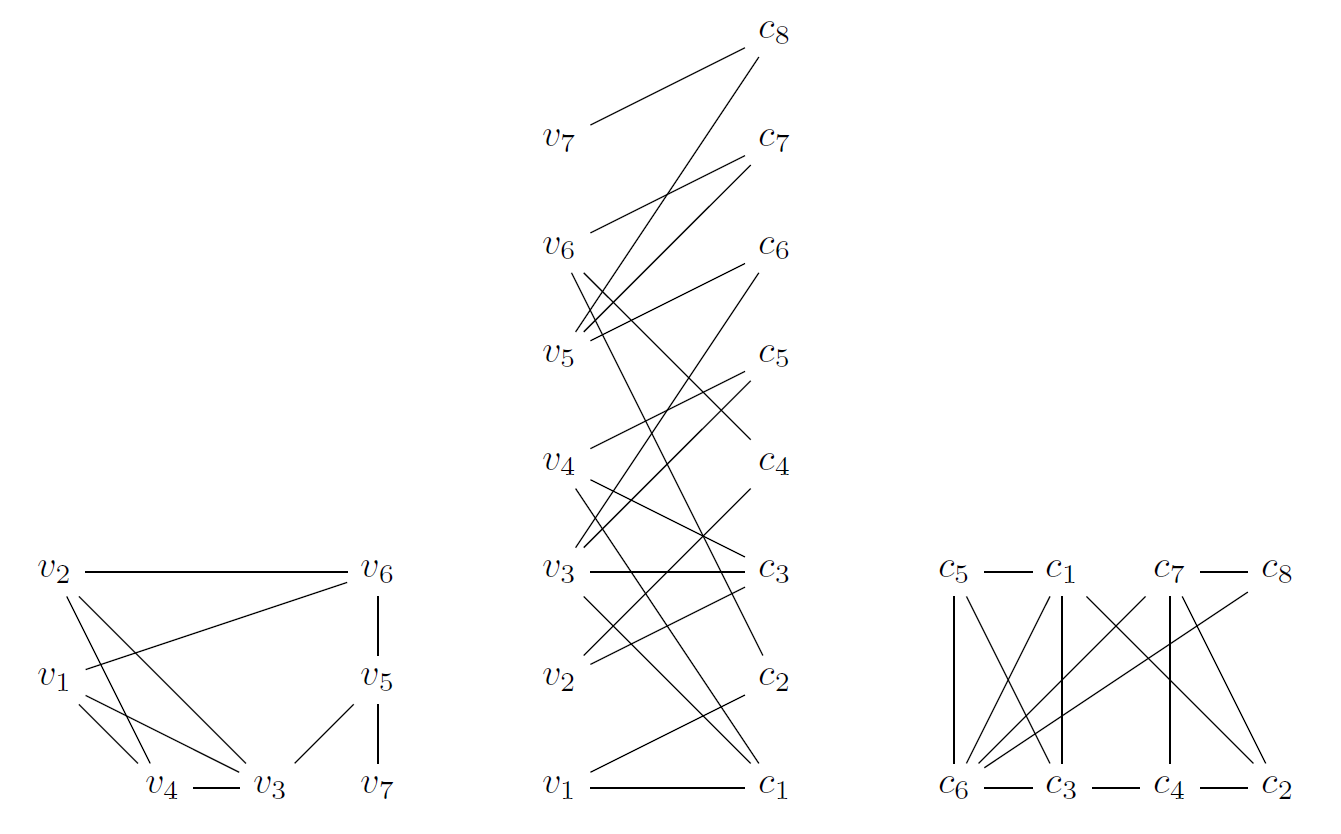
\includegraphics[height=0.5\textheight]{images/DAGraphs.png}
		\caption{The primal (left), incidence (middle) and dual (right) graph}
	\end{figure}
%\footnotesize{Equivalent CNF}
%{\tiny $(\neg \text{v1}\lor \neg \text{v3})\land (\neg \text{v1}\lor \text{v6})\land (\text{v1}\lor \neg \text{v4})\land (\neg \text{v2}\lor \neg \text{v5})\land (\neg \text{v2}\lor \text{v6})\land (\neg \text{v3}\lor \neg \text{v4})\land (\neg \text{v3}\lor \text{v5})\land (\neg \text{v5}\lor \neg \text{v6})\land (\text{v5}\lor \text{v7})$}

\end{frame}

%%
\subsection[TD]{Tree decomposition}
\begin{frame}
\frametitle{Tree Decompositions}
{\color{blue}\emph{Parameterized Complexity and its Applications in Practice} \\
From Foundations to Implementations \\
Johannes K. Fichte \\
TU Dresden, Germany \\
Jakarta, Indonesia \\
{Summer 2019 (May 6th - May 16th)}
}
pages 162-174\\
\bigskip
\emph{Backup}: VC tree vs graph - example p69, 128 
\end{frame}
%{
%	\setbeamercolor{background canvas}{bg=}
%	\includepdf[pages=162-174]{"images/Lecture_pcgp_Summer_2019.pdf"}
%}
%%%%%%%%%%%%%%%%%%%%%%%
\section{implementations}
\subsection{gpusat1}
\begin{frame}
	\frametitle{gpuSAT1}
	\begin{figure}
		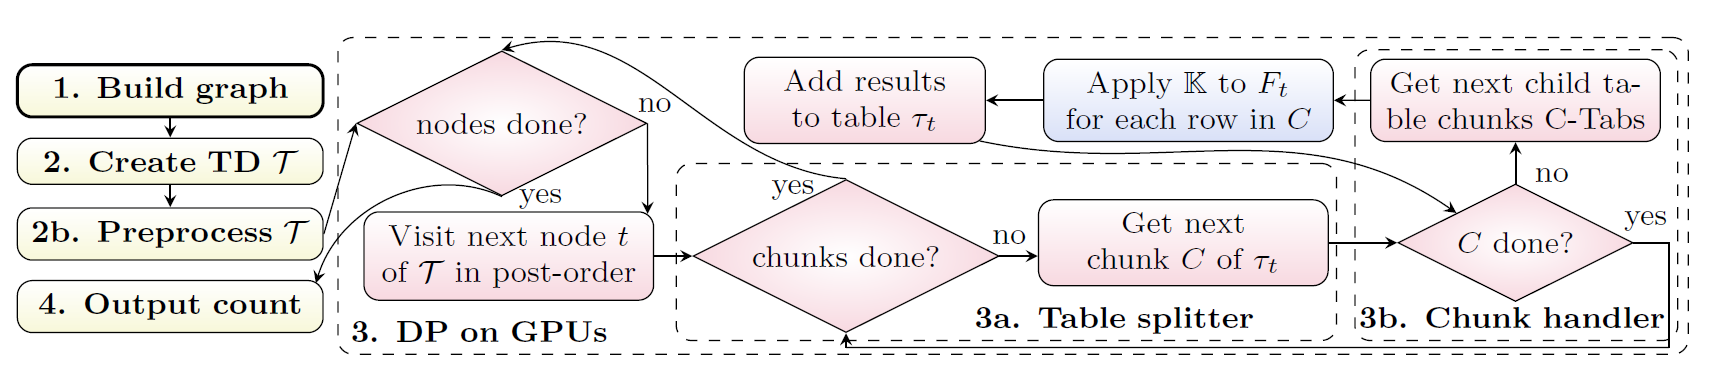
\includegraphics[width=0.8\linewidth]{images/DADPonGPU.png}
		\caption{DP algorithm on the GPU}
	\end{figure}

	\begin{minipage}{0.49\textwidth}
		\begin{itemize}
			\item OpenCL
			\item Two operations between bags
		\end{itemize}
	\end{minipage}
\begin{minipage}{0.49\textwidth}
		\begin{figure}
		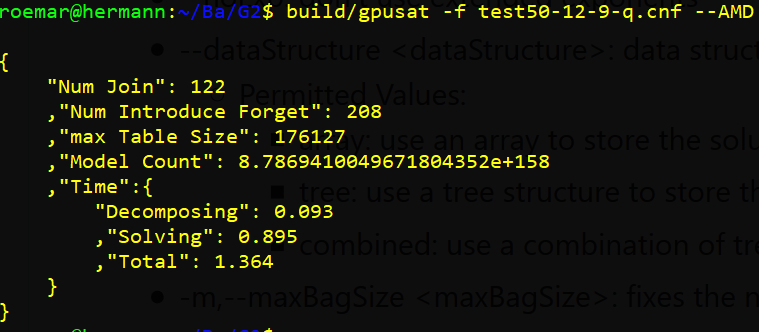
\includegraphics[width=\linewidth]{images/Hermann gpusat test50 running.png}
		\caption{Example output format from gpuSAT}
	\end{figure}
\end{minipage}
	github: \url{https://github.com/daajoe/GPUSAT}
\end{frame}
%%
\subsection{gpusat2}
\begin{frame}
	\frametitle{gpuSAT2 - Improving Upon Previous Ideas }
	%Architecture of our DP-based solver for parallel execution. Yellow colored
	%boxes indicate tasks that are required as initial step for the DP-run or to nally read the
	%model count from the computed results. The parts framed by a dashed box illustrate the
	%DP-part. Boxes colored in red indicate computations that run on the CPU. Boxes colored
	%in blue indicate computations that are executed on the GPU (with waiting CPU).
	\begin{figure}
		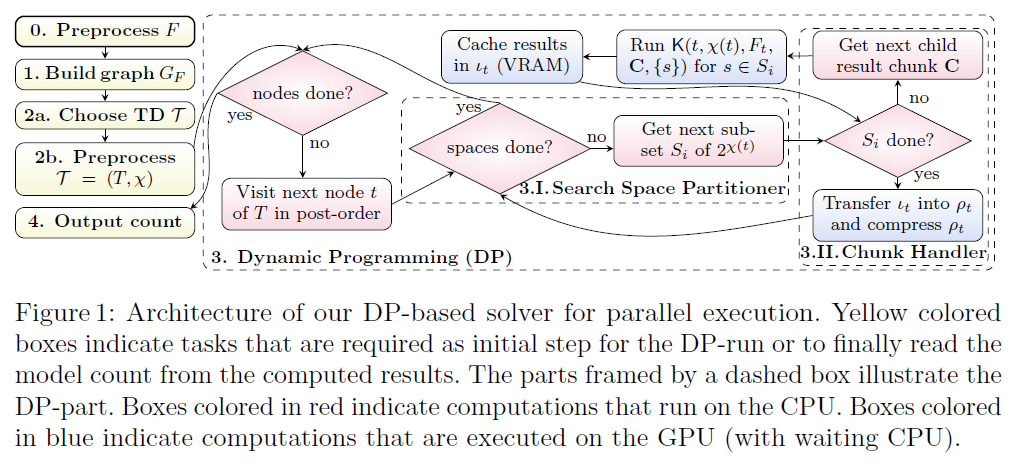
\includegraphics[height=0.3\textheight]{images/gpusat2DP.png}
	\end{figure}
\begin{minipage}{0.49\textwidth}
	\begin{itemize}

		\item only primal graph { \small (simpler solving DP)}
		\item customized tree decompositions
		\item adapted memory-management
		\item improved precision handling

	\end{itemize}
\end{minipage}
\begin{minipage}{0.49\textwidth}
	%Runtime for the top 5 sequential and all parallel solvers over all the #Sat
	%instances with pmc preprocessor. The x-axis refers to the number of instances and the
	%y-axis depicts the runtime sorted in ascending order for each solver individually.
	\begin{figure}
		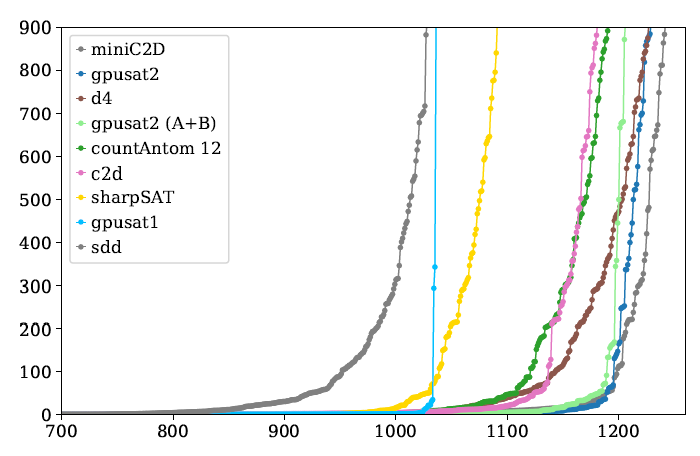
\includegraphics[width=\linewidth]{images/gpusat2Runtime.png}
	\end{figure}
\end{minipage}

\end{frame}
%%
\subsection{dpdb}
\begin{frame}
	\frametitle{dpdb}
	{\color{blue}Using databases for intermediate results} \medskip\\
	%The idea of dpdb is to use database
	%management systems (DBMS) for table manipulation, which makes it (1) easy
	%and elegant to perform rapid prototyping for problems, and (2) allows to leverage
	%from decades of database theory and database system tuning. It turned out that
	%all the cases that occur in dynamic programming can be handled quite elegantly
	%with plain SQL queries. Our system dpdb can be used for both decision and
	%counting problems, thereby also considering optimization. We see our system
	%particularly well-suited for counting problems, especially, since it was shown
	%that for model counting (#Sat) instances of practical relevance typically have
	%small treewidth [23]. In consequence, we carried out preliminary experiments
	%on publicly available instances for
	\begin{minipage}{0.1\textwidth}
		\hfill
	\end{minipage}
	\begin{minipage}{0.35\textwidth}
	\begin{itemize}
		\item SAT
		\item \#SAT
		\item \#o-Coloring
		\item Vertex cover
	\end{itemize}
\end{minipage}\hfill
\begin{minipage}{0.54\textwidth}
	
	\begin{figure}
		\centering\hfill
		\begin{subfigure}[b]{\textwidth}
			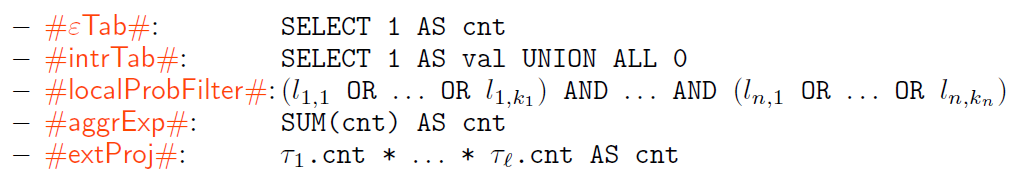
\includegraphics[width=\linewidth]{images/dpdbSSat.png}
			\caption{Problem \#SAT}

		\end{subfigure}\hfill\\
	\begin{subfigure}[b]{\textwidth}
		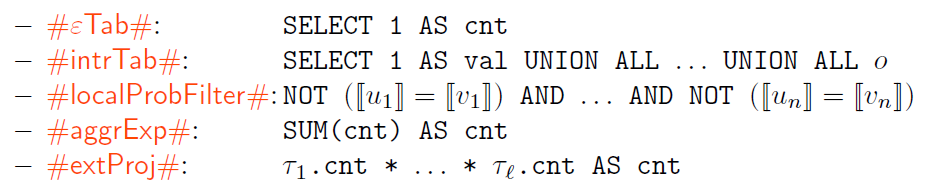
\includegraphics[width=0.8\linewidth]{images/dpdbOCol.png}
		\caption{Problem \#o-Col}

	\end{subfigure}\hfill\\
\begin{subfigure}[b]{\textwidth}
	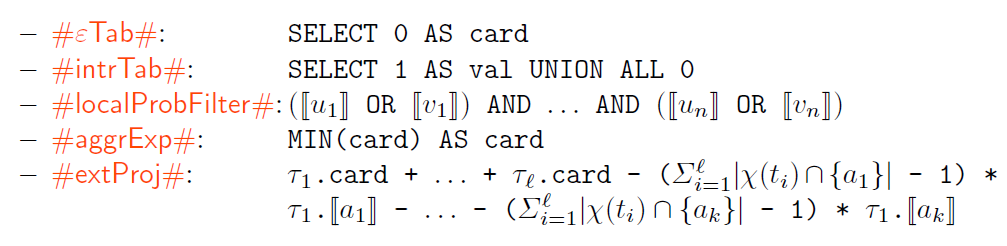
\includegraphics[width=0.8\linewidth]{images/dpdbMinVC.png}
	\caption{Problem MinVC}

\end{subfigure}
	\end{figure}

\end{minipage}
\medskip \\
github: \url{https://github.com/hmarkus/dp_on_dbs}
\end{frame}
\begin{frame}
	\medskip
	\frametitle{dpdb - Benchmark}
	{\color{blue}Performance of all three programs on \#SAT instances:} \medskip\\
	\begin{figure}
		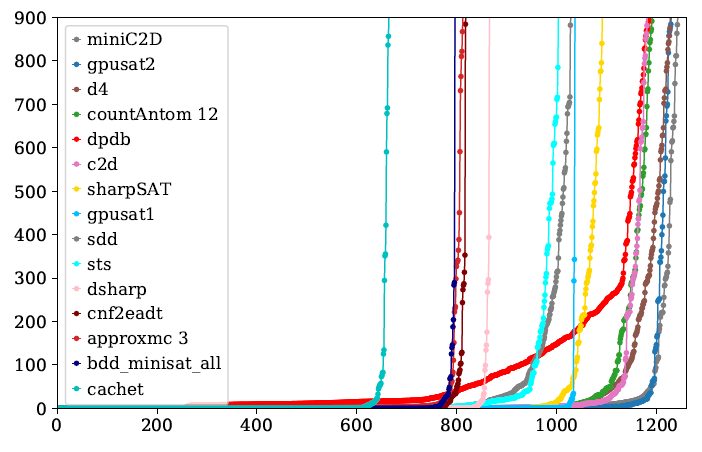
\includegraphics[width=0.8\linewidth]{images/dpdbRuntime.png}
	\end{figure}
\end{frame}

%%%%%%%%%%%%%%%%%%%%%%%
\section{Visualization}
\subsection{Handcrafted}
\begin{frame}
	\frametitle{Existing Visualization}
	\begin{figure}
		\centering
		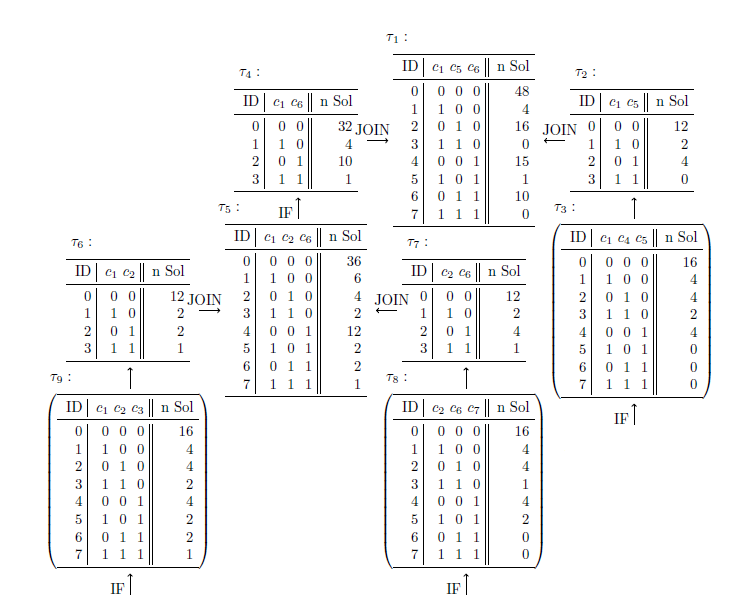
\includegraphics[width=0.6\linewidth]{images/DualDA43.png}
		\caption{Handcrafted \#SAT example-run from Markus Zisser\footnote{"Solving \#SAT on the GPU with Dynamic Programming and OpenCL",\\ Diploma Markus Zisser 2018 Technische Universit�t Wien, p.33}}
		\label{fig:dualda43}
	\end{figure}

\end{frame}
\begin{frame}
	\frametitle{Existing Visualization}
	\begin{figure}
		\centering
		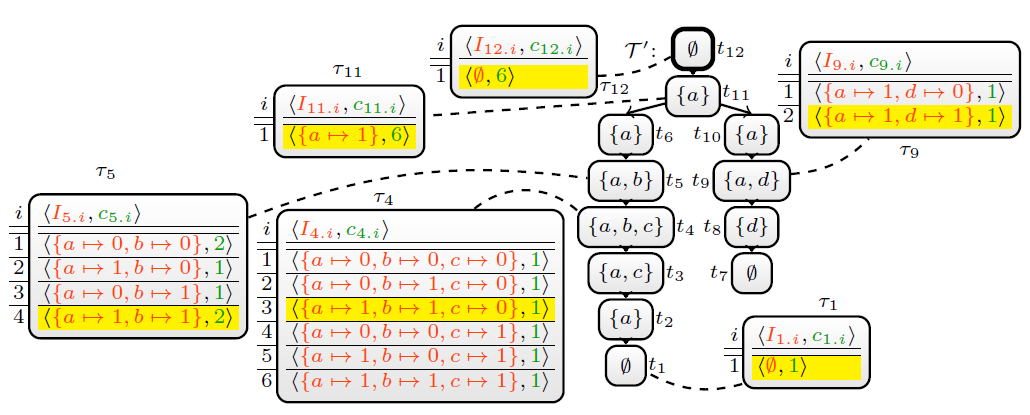
\includegraphics[width=\linewidth]{images/dpdbVisuSat.png}
		\caption{Handcrafted \#SAT example-run from dpdb\footnote{"Exploiting Database Management Systems and Treewidth for Counting",\\ Fichte, Hecher, Thier, Woltran} }
		\label{fig:dpdbVisuSat}
	\end{figure}
	
	
\end{frame}

%%%%%%%%%%%%%%%%%%%%%%%
\section{Further Visualization}
\begin{frame}
\frametitle{Creating Visualization for:}
\begin{minipage}{0.44\textwidth}
	\emph{Improving}
	\begin{itemize}
		\item examples for students 
		\item debugging and improving interaction of complex data-structures
		\item hotspots
	\end{itemize}\medskip

\end{minipage}
\begin{minipage}{0.55\textwidth}
	\begin{figure}
		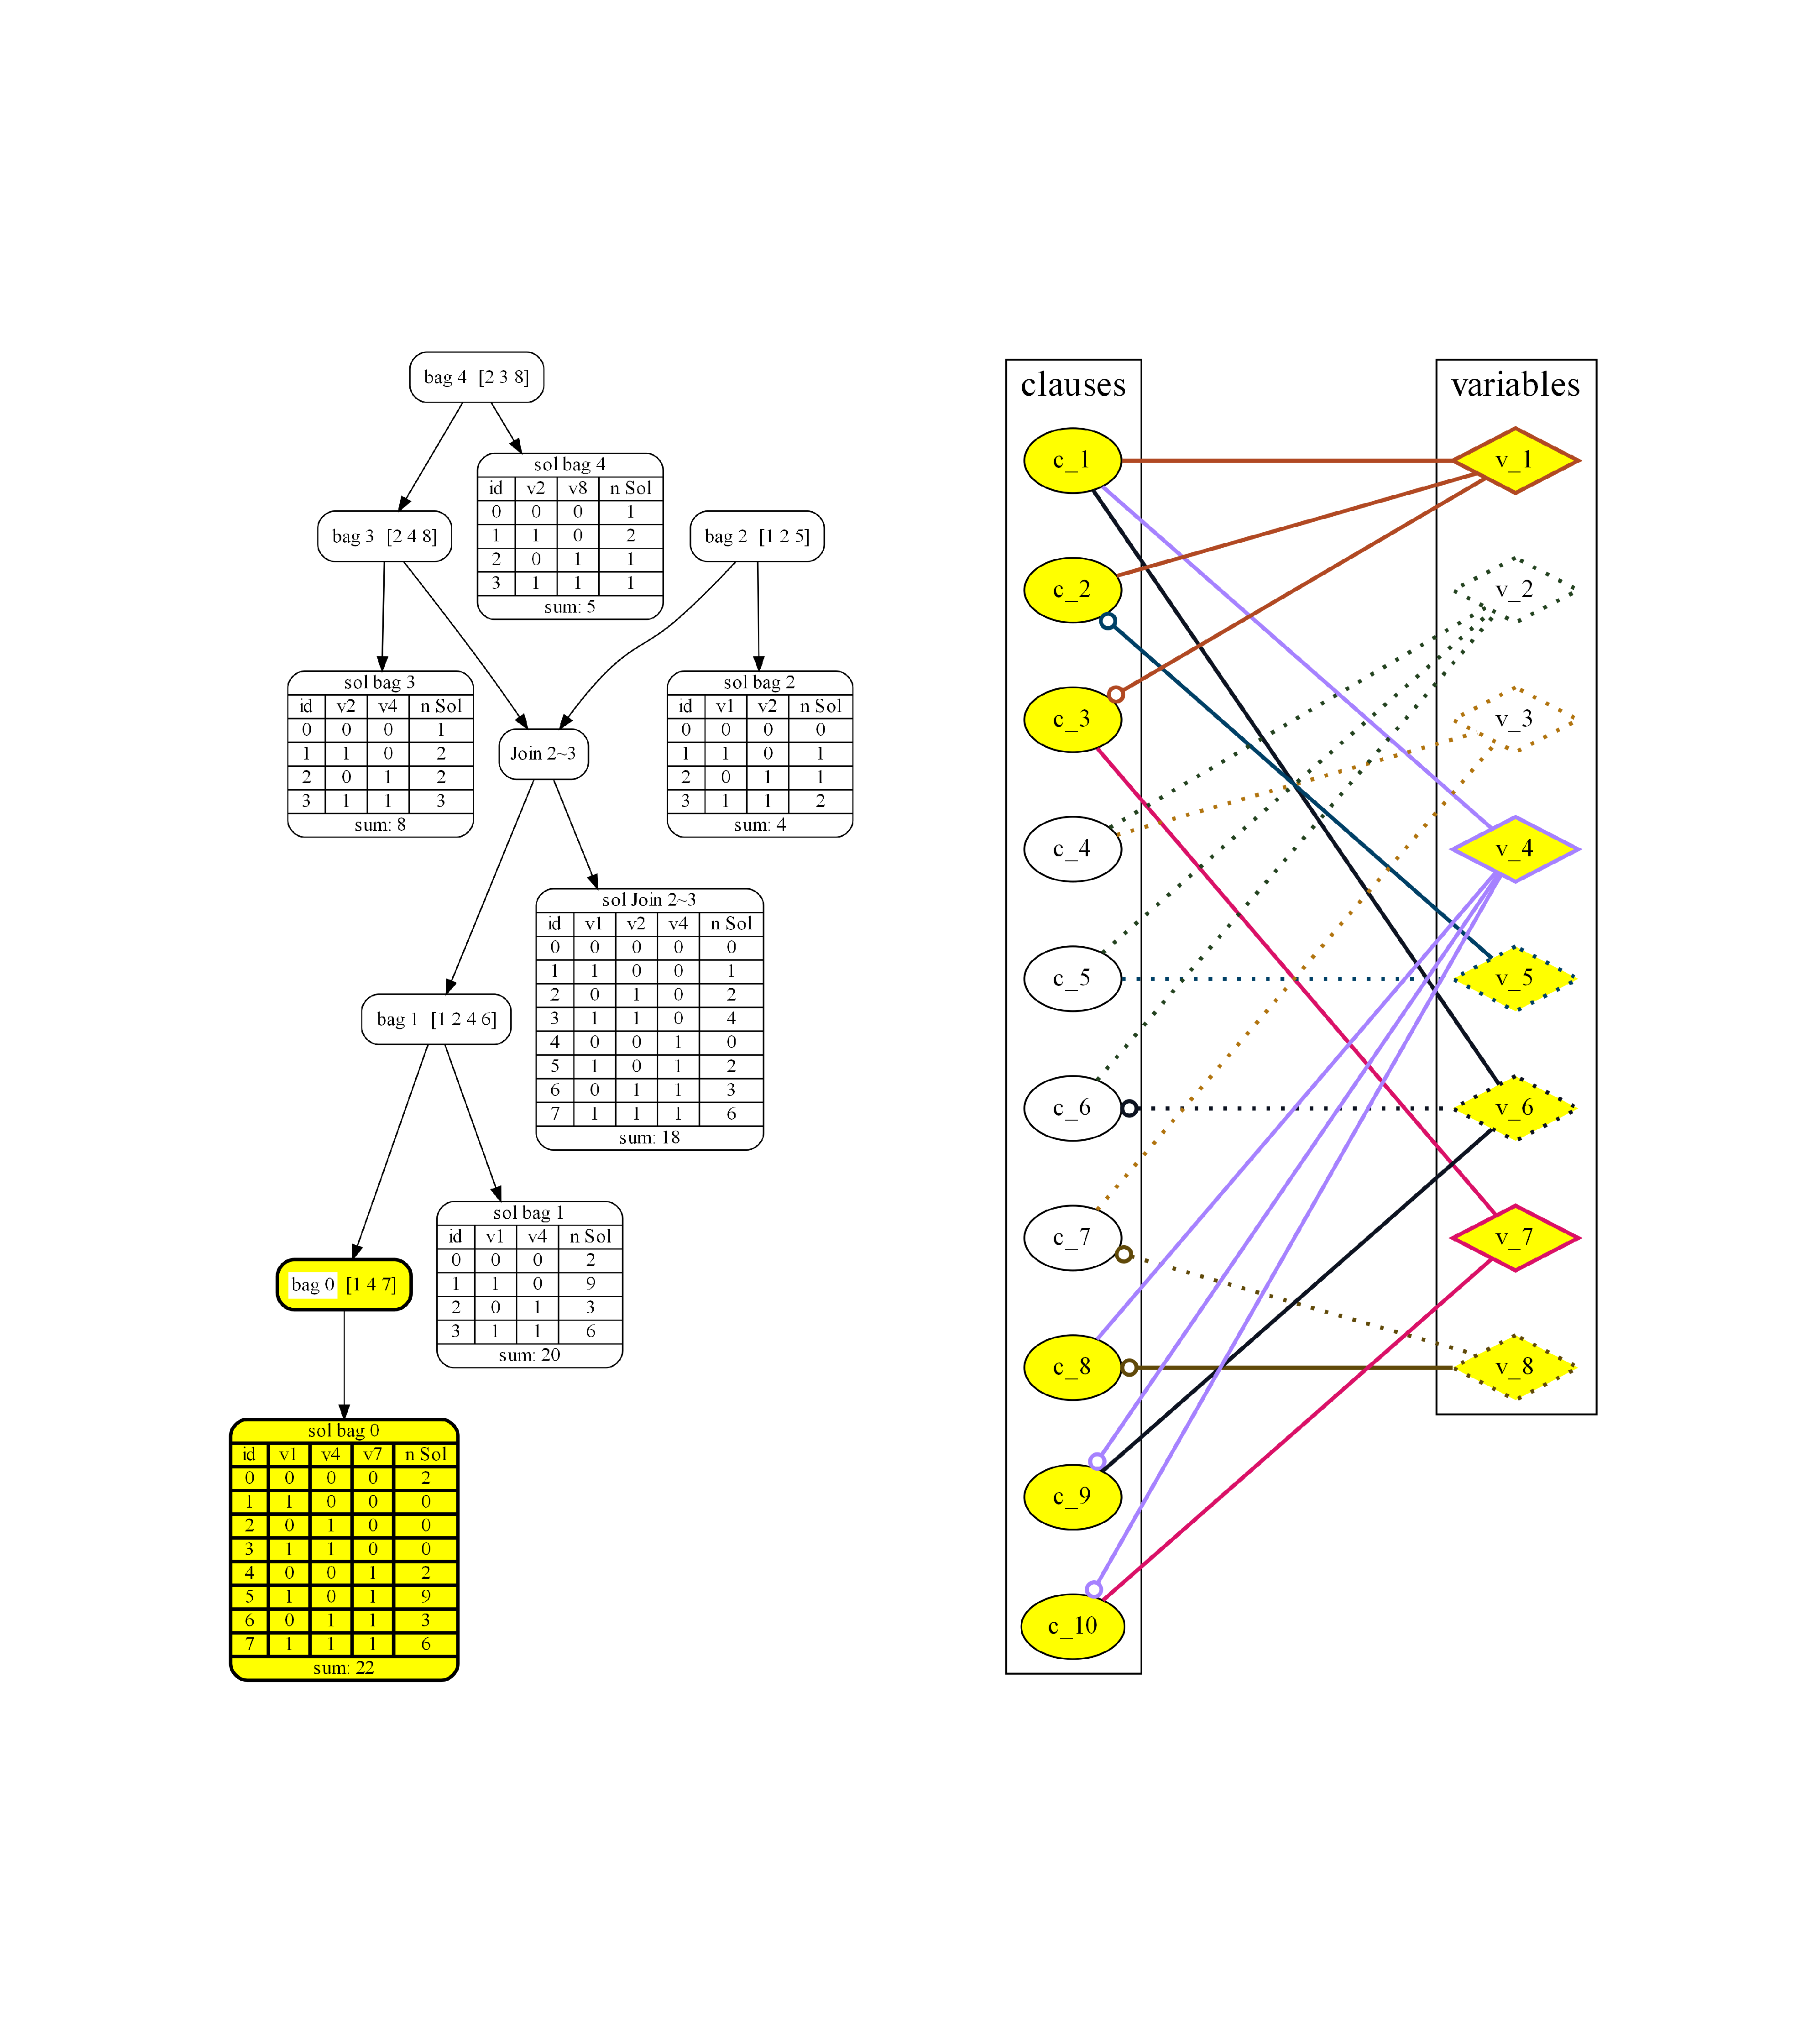
\includegraphics[width=\linewidth]{images/combined8.png}
	\end{figure}
\end{minipage}

\end{frame}

%%%%%%%%%%%%%%%%%%%%%%%
\section{Outlook}
\begin{frame}
	\frametitle{Outlook}
	\medskip
	{\color{blue}What can I do?\\}	
	\medskip
	\centering
	Visualization\medskip\\
	\begin{itemize}
		\item customizable output and interactive visualization
		\item possibility of generalizing the underlying graph structure \textit{(Hypergraphs)}
		\item reference impl. in CUDA of gpuSAT2 
	\end{itemize}
\end{frame}

%%%%%%%%%%%%%%%%%%%%%%%

\bgroup
\setbeamercolor{background canvas}{bg=black}
\begin{frame}[plain]{}
\end{frame}
\egroup

\end{document}
